
%%%%%%%%%%%%%%%%%%%%%%%%%%%%%%%%%%%%%%%%%%%%%%%%%%%%%%%%%%%%%%%%%%%%%%%%%%%%%%%%
%% ************************************************************************** %%
%% *                                Settings                                * %%
%% ************************************************************************** %%
%%%%%%%%%%%%%%%%%%%%%%%%%%%%%%%%%%%%%%%%%%%%%%%%%%%%%%%%%%%%%%%%%%%%%%%%%%%%%%%%
\documentclass{tron}

\loadglsentries{gls}
\glsaddall
\addbibresource{reference}
\usepackage{xcolor}  % Coloured text etc.
% fancy note style
% STYLE NOTES : v2.0
% additional fancy boxes
\usepackage[framemethod=TikZ]{mdframed}
%\usepackage{amsthm}

% gray color indicates [OPTIONAL READING]

%%%%%%%%%%%%%%%%%%%%%%%%%%%%%%
%Note
\newenvironment{note}[3][]{%
	\ifstrempty{#1}%
	{\mdfsetup{%
	frametitle={%
	\tikz[baseline=(current bounding box.east),outer sep=0pt]
	\node[anchor=east,rectangle,fill=#2]
	{\strut Note};}}
	}%
	{\mdfsetup{%
	frametitle={%
	\tikz[baseline=(current bounding box.east),outer sep=0pt]
	\node[anchor=east,rectangle,fill=#2]
	{\strut #1};}}%
	}%
	\mdfsetup{innertopmargin=0pt,skipabove=5pt,linecolor=#2,%
		linewidth=2pt,topline=true,%
		frametitleaboveskip=\dimexpr-\ht\strutbox\relax,
		backgroundcolor={white!90!#2}}
	\begin{mdframed}[]\relax%
	\label{#3}}{\end{mdframed}
}
\Crefname{note}{Note}{notes}

\newcommand{\createnoteenv}[6]{
	\refstepcounter{#6}%
	\ifstrempty{#1}%
	{\mdfsetup{%
	frametitle={%
	\tikz[baseline=(current bounding box.east),outer sep=0pt]
	\node[anchor=east,rectangle,fill=#3]
	{\strut #4~#5};}}
	}%
	{
		\mdfsetup{%
			frametitle={%
				\tikz[baseline=(current bounding box.east),outer sep=0pt]
				\node[anchor=east,rectangle,fill=#3]
				{\strut #4~#5:~#1};
			}
		}%
	}%
	\mdfsetup{innertopmargin=0pt,skipabove=5pt,linecolor=#3,%
	linewidth=2pt,topline=true,%
	frametitleaboveskip=\dimexpr-\ht\strutbox\relax,
	backgroundcolor={white!90!#3}}
	\begin{mdframed}[]\relax%
	\label{#2}
}

%%%%%%%%%%%%%%%%%%%%%%%%%%%%%%
%Definition
\newcounter{definition}[section] \setcounter{definition}{0}
\renewcommand{\thedefinition}{\arabic{section}.\arabic{definition}}
\newenvironment{definition}[2][]{%
	\createnoteenv{#1}{#2}{blue!40}{Definition}{\thedefinition}{definition}%
}{\end{mdframed}}
\newenvironment{definition*}[2][]{%
	\createnoteenv{#1}{#2}{gray!40}{Definition}{\thedefinition}{definition}%
}{\end{mdframed}}
\Crefname{definition}{Definition}{definitions}


%%%%%%%%%%%%%%%%%%%%%%%%%%%%%%
%theoremrem
\newcounter{theorem}[section] \setcounter{theorem}{0}
\renewcommand{\thetheorem}{\arabic{section}.\arabic{theorem}}
\newenvironment{theorem}[2][]{%
	\createnoteenv{#1}{#2}{cyan!40}{Theorem}{\thetheorem}{theorem}%
}{\end{mdframed}}
\newenvironment{theorem*}[2][]{%
	\createnoteenv{#1}{#2}{gray!40}{Theorem}{\thetheorem}{theorem}%
}{\end{mdframed}}
\Crefname{theorem}{Theorem}{theorems}

%%%%%%%%%%%%%%%%%%%%%%%%%%%%%%
%Proof
\newcounter{proof}[section]\setcounter{proof}{0}
\renewcommand{\theproof}{\arabic{section}.\arabic{proof}}
\newenvironment{proof}[2][]{%
	\createnoteenv{#1}{#2}{red!20}{Proof}{\theproof}{proof}%
}{\end{mdframed}}
\newenvironment{proof*}[2][]{%
	\createnoteenv{#1}{#2}{gray!40}{Proof}{\theproof}{proof}%
}{\end{mdframed}}
\Crefname{proof}{Proof}{proofs}


%%%%%%%%%%%%%%%%%%%%%%%%%%%%%%
%Alert
\newcounter{alert}[section]\setcounter{alert}{0}
\renewcommand{\thealert}{\arabic{section}.\arabic{alert}}
\newenvironment{alert}[2][]{%
	\createnoteenv{#1}{#2}{red!80}{Alert}{\thealert}{alert}%
}{\end{mdframed}}
\newenvironment{alert*}[2][]{%
	\createnoteenv{#1}{#2}{gray!40}{Alert}{\thealert}{alert}%
}{\end{mdframed}}
\Crefname{alert}{Alert}{alerts}

%%%%%%%%%%%%%%%%%%%%%%%%%%%%%%
%Answer
\newcounter{answer}[section]\setcounter{answer}{0}
\renewcommand{\theanswer}{\arabic{section}.\arabic{answer}}
\newenvironment{answer}[2][]{%
	\createnoteenv{#1}{#2}{orange!60}{Answer}{\theanswer}{answer}%
}{\end{mdframed}}
\newenvironment{answer*}[2][]{%
	\createnoteenv{#1}{#2}{gray!40}{Answer}{\theanswer}{answer}%
}{\end{mdframed}}
\Crefname{answer}{Answer}{answers}

%%%%%%%%%%%%%%%%%%%%%%%%%%%%%%
%Remark
\newcounter{remark}[section]\setcounter{remark}{0}
\renewcommand{\theremark}{\arabic{section}.\arabic{remark}}
\newenvironment{remark}[2][]{%
	\createnoteenv{#1}{#2}{orange!40}{Remark}{\theremark}{remark}%
}{\end{mdframed}}
\newenvironment{remark*}[2][]{%
	\createnoteenv{#1}{#2}{gray!40}{Remark}{\theremark}{remark}%
}{\end{mdframed}}
\Crefname{remark}{Remark}{remarks}


%%%%%%%%%%%%%%%%%%%%%%%%%%%%%%%
%%Example
%\newcounter{example}[section]\setcounter{example}{0}
%\renewcommand{\theexample}{\arabic{section}.\arabic{example}}
%\newenvironment{example}[2][]{%
%	\createnoteenv{#1}{#2}{blue!40!cyan!20}{Example}{\theexample}{example}%
%}{\end{mdframed}}
%\newenvironment{example*}[2][]{%
%	\createnoteenv{#1}{#2}{gray!40}{Example}{\theexample}{example}%
%}{\end{mdframed}}

%%%%%%%%%%%%%%%%%%%%%%%%%%%%%%
%Algorithm
\newcounter{algo}[section]\setcounter{algo}{0}
\renewcommand{\thealgo}{\arabic{algo}.\arabic{algo}}
\newenvironment{algo}[2][]{%
	\createnoteenv{#1}{#2}{yellow!90!brown!60}{Algorithm}{\thealgo}{algo}%
}{\end{mdframed}}
\newenvironment{algo*}[2][]{%
	\createnoteenv{#1}{#2}{gray!40}{Algorithm}{\thealgo}{algo}%
}{\end{mdframed}}
\Crefname{algo}{Algorithm}{algos}

%%%%%%%%%%%%%%%%%%%%%%%%%%%%%%
% CS480 - Exercise
%\setlength{\parskip}{1cm}
%\setlength{\parindent}{1cm}

%\tikzstyle{titregris} =
%[draw=gray,fill=white, shading = exersicetitle, %
%text=gray, rectangle, rounded corners, right,minimum height=.3cm]
%\pgfdeclarehorizontalshading{exersicebackground}{100bp}
%{color(0bp)=(green!40); color(100bp)=(black!5)}
%\pgfdeclarehorizontalshading{exersicetitle}{100bp}
%{color(0bp)=(red!40);color(100bp)=(black!5)}
%\newcounter{exercise}
%\renewcommand*\theexercise{exercice \textbf{Exercice}~n\arabic{exercise}}
%\makeatletter
%\def\mdf@@exercisepoints{}%new mdframed key:
%\define@key{mdf}{exercisepoints}{%
%\def\mdf@@exercisepoints{#1}
%}
%
%\mdfdefinestyle{theoremstyle}{%
%outerlinewidth=0.01em,linecolor=black,middlelinewidth=0.5pt,%
%frametitlerule=true,roundcorner=2pt,%
%apptotikzsetting={\tikzset{mfframetitlebackground/.append style={%
%shade,left color=white, right color=blue!20}}},
%frametitlerulecolor=black,innertopmargin=1\baselineskip,%green!60,
%innerbottommargin=0.5\baselineskip,
%frametitlerulewidth=0.1pt,
%innertopmargin=0.7\topskip,skipabove={\dimexpr0.2\baselineskip+0.1\topskip\relax},
%frametitleaboveskip=1pt,
%frametitlebelowskip=1pt
%}
%\mdtheorem[style=theoremstyle]{exercise}{\textbf{Exercise}}

\newcounter{exercise}[section]\setcounter{exercise}{0}
\renewcommand{\theexercise}{\arabic{exercise}}
\newenvironment{exercise}[2][]{%
	\createnoteenv{#1}{#2}{gray!40}{Exercise}{\theexercise}{exercise}%
}{\end{mdframed}}
\newenvironment{exercise*}[2][]{%
	\createnoteenv{#1}{#2}{gray!40}{Exercise}{\theexercise}{exercise}%
}{\end{mdframed}}

\Crefname{exercise}{Exercise}{exercises}


%%%%%%%%%%%%%%%%%%%%%%%%%%%%%%
%Examples
% {

%     \section{Theorem and lemma examples with title}
%     \begin{theorem}[Pythagoras' theorem]{theorem:pythagoras}
%     In a right triangle, the square of the hypotenuse is equal to the sum of the squares of the catheti.
%     \[a^2+b^2=c^2\]
%     \end{theorem}
%     In mathematics, the Pythagorean theorem, also known as Pythagoras' theorem (see theorem \ref{theorem:pythagoras}), is a relation in Euclidean geometry among the three sides of a right triangle.
%     
%     \begin{definition}[B\'ezout's identity]{def:bezout}
%     Let $a$ and $b$ be nonzero integers and let $d$ be their greatest common divisor. Then there exist integers $x$ and $y$ such that:
%     \[ax+by=d\]
%     \end{definition}
%     This is a reference to Bezout's lemma \ref{def:bezout}
%     
%     
%     \section{Theorem and proof examples without title}
%     
%     \begin{theorem}[]{theorem:theorem1}
%     There exist two irrational numbers $x$, $y$ such that $x^y$ is rational.
%     \end{theorem}
%     
%     \begin{proof}[]{proof:proof1}
%     If $x=y=\sqrt{2}$ is an example, then we are done; otherwise $\sqrt{2}^{\sqrt{2}}$ is irrational, in which case taking $x=\sqrt{2}^{\sqrt{2}}$ and $y=\sqrt{2}$ gives us:
%     \[\bigg(\sqrt{2}^{\sqrt{2}}\bigg)^{\sqrt{2}}=\sqrt{2}^{\sqrt{2}\sqrt{2}}=\sqrt{2}^{2}=2.\]
%     \end{proof}
%
%     \begin{alert}[]{alert:alert1}
%     If $x=y=\sqrt{2}$ is an example, then we are done; otherwise $\sqrt{2}^{\sqrt{2}}$ is irrational, in which case taking $x=\sqrt{2}^{\sqrt{2}}$ and $y=\sqrt{2}$ gives us:
%     \[\bigg(\sqrt{2}^{\sqrt{2}}\bigg)^{\sqrt{2}}=\sqrt{2}^{\sqrt{2}\sqrt{2}}=\sqrt{2}^{2}=2.\]
%     \end{alert}
%     
%     \begin{remark}[]{alert:alert1}
%     If $x=y=\sqrt{2}$ is an example, then we are done; otherwise $\sqrt{2}^{\sqrt{2}}$ is irrational, in which case taking $x=\sqrt{2}^{\sqrt{2}}$ and $y=\sqrt{2}$ gives us:
%     \[\bigg(\sqrt{2}^{\sqrt{2}}\bigg)^{\sqrt{2}}=\sqrt{2}^{\sqrt{2}\sqrt{2}}=\sqrt{2}^{2}=2.\]
%     \end{remark}
%     
%     
%          \begin{exercise}[]{alert:alert1}
%     If $x=y=\sqrt{2}$ is an example, then we are done; otherwise $\sqrt{2}^{\sqrt{2}}$ is irrational, in which case taking $x=\sqrt{2}^{\sqrt{2}}$ and $y=\sqrt{2}$ gives us:
%     \[\bigg(\sqrt{2}^{\sqrt{2}}\bigg)^{\sqrt{2}}=\sqrt{2}^{\sqrt{2}\sqrt{2}}=\sqrt{2}^{2}=2.\]
%     \end{exercise}
%     
%     \begin{algo}[]{algorithm:alert1}
%     If $x=y=\sqrt{2}$ is an example, then we are done; otherwise $\sqrt{2}^{\sqrt{2}}$ is irrational, in which case taking $x=\sqrt{2}^{\sqrt{2}}$ and $y=\sqrt{2}$ gives us:
%     \[\bigg(\sqrt{2}^{\sqrt{2}}\bigg)^{\sqrt{2}}=\sqrt{2}^{\sqrt{2}\sqrt{2}}=\sqrt{2}^{2}=2.\]
%     \end{algo}
%     
%     \begin{note}[Goal]{pink}{note:goal}
%     If $x=y=\sqrt{2}$ is an example, then we are done; otherwise $\sqrt{2}^{\sqrt{2}}$ is irrational, in which case taking $x=\sqrt{2}^{\sqrt{2}}$ and $y=\sqrt{2}$ gives us:
%     \[\bigg(\sqrt{2}^{\sqrt{2}}\bigg)^{\sqrt{2}}=\sqrt{2}^{\sqrt{2}\sqrt{2}}=\sqrt{2}^{2}=2.\]
%     \end{note}

% }
%\usepackage{lipsum}                     % Dummytext
\usepackage{xargs}                      % Use more than one optional parameter in a new commands
\usepackage[colorinlistoftodos,prependcaption,textsize=normalsize]{todonotes}
%
\newcommandx{\unsure}[2][1=]{\todo[linecolor=red,backgroundcolor=red!25,bordercolor=red,#1]{#2}}
\newcommandx{\change}[2][1=]{\todo[linecolor=blue,backgroundcolor=blue!25,bordercolor=blue,#1]{#2}}
\newcommandx{\info}[2][1=]{\todo[linecolor=OliveGreen,backgroundcolor=OliveGreen!25,bordercolor=OliveGreen,#1]{#2}}
\newcommandx{\improvement}[2][1=]{\todo[linecolor=Plum,backgroundcolor=Plum!25,bordercolor=Plum,#1]{#2}}
\newcommandx{\thiswillnotshow}[2][1=]{\todo[disable,#1]{#2}}
%
\preto\printlistoftodos{
    \listoftodos[Todo List]
}

% EXAMPLES:
    % \todo[inline]{The original todo note withouth changed colours.\newline Here's another line.}
    % \lipsum[11]\unsure{Is this correct?}\unsure{I'm unsure about also!}
    % \lipsum[11]\change{Change this!}
    % \lipsum[11]\info{This can help me in chapter seven!}
    % \lipsum[11]\improvement{This really needs to be improved!\newline\newline What was I thinking?!}
    % \lipsum[11]
    % \thiswillnotshow{This is hidden since option `disable' is chosen!}
    % \improvement[inline]{The following section needs to be rewritten!}
    % \lipsum[11]
    % \newpage
    % \listoftodos[Notes]
%%%  Equation Condition
\newenvironment{eqconditions}
  {\par\vspace{\abovedisplayskip}\noindent\begin{tabular}{>{$}l<{$} @{${}={}$} l}}
  {\end{tabular}\par\vspace{\belowdisplayskip}}
\newenvironment{eqconditions*}
  {\noindent\begin{tabular}{>{$}l<{$} @{${}={}$} l}}
  {\end{tabular}}
%%% introduce 4th depth with \paragraph command
\usepackage{titlesec}
\setcounter{secnumdepth}{4}
\titleformat{\paragraph}
{\normalfont\normalsize\bfseries}{\theparagraph}{1em}{}
\titlespacing*{\paragraph}
{0pt}{3.25ex plus 1ex minus .2ex}{1.5ex plus .2ex}

%%% enumeration reference
% constraint
\newlist{constraint-list}{enumerate}{1}
\setlist[constraint-list,1]{leftmargin=*, label= \Roman*}
\creflabelformat{Constraint}{#2#1#3}
\crefname{constraint-listi}{Constraint}{position}
% criteria
\newlist{criteria-list}{enumerate}{1}
\setlist[criteria-list,1]{leftmargin=*, label= \Roman*}
\creflabelformat{Criterion}{#2#1#3}
\crefname{criteria-listi}{Criterion}{position}
% property
\newlist{property-list}{enumerate}{1}
\setlist[property-list,1]{leftmargin=*, label= \Roman*}
\creflabelformat{Property}{#2#1#3}
\crefname{property-listi}{Property}{position}
% assumption
\newlist{assumption-list}{enumerate}{1}
\setlist[assumption-list,1]{leftmargin=*, label= \Roman*}
\creflabelformat{Assumption}{#2#1#3}
\crefname{assumption-listi}{Assumption}{position}

% custom math command
\newcommand{\unit}[1]{\left[\si{#1}\right]}

% additional math packages
\usepackage{physics}
\usepackage{cancel}

% TODO Flags
\newcommand\TODO[1]{{\textcolor{red}{\textbf{#1}}}}
\newcommand\COMMENT[1]{\hl{#1}}

% Custom Format
% \usepackage{float}
% \usepackage[table]{xcolor}
% \usepackage{soul}
\usepackage{multirow}
\usepackage{caption} 
\captionsetup[table]{skip=3pt}
\captionsetup[figure]{skip=0pt}
\titlespacing*{\section}
{0pt}{10pt}{3pt}
\titlespacing*{\subsection}
{0pt}{8pt}{3pt}
\titlespacing*{\subsubsection}
{0pt}{8pt}{3pt}
%hide the highlight box
\hypersetup{
    colorlinks,
    linkcolor={black!50!black},
    citecolor={black!50!blue},
    urlcolor={black!80!black}
}%hide the highlight box

% table formatting
% \setlength{\arrayrulewidth}{1mm}
% \setlength{\tabcolsep}{18pt}
% \renewcommand{\arraystretch}{2.5}
\usepackage{array}
\newcolumntype{C}[1]{>{\centering\let\newline\\\arraybackslash\hspace{0pt}}m{#1}}

% custom math symbol
%% CS 480 %%
\newcommand{\bm}[1]{\mathbf{#1}}
%%%%%%%%%%%%
\newcommand{\RR}{\mathds{R}}
\newcommand{\Id}{\mathbb{I}}
\newcommand{\NN}{\mathds{N}}
\newcommand{\sign}{\mathop{\mathrm{sign}}}
\newcommand{\diag}{\mathop{\mathrm{diag}}}
\newcommand{\argmin}{\mathop{\mathrm{argmin}}}
\newcommand{\zero}{\mathbf{0}}
\newcommand{\one}{\mathbf{1}}
\newcommand{\av}{\mathbf{a}}
\newcommand{\bv}{\mathbf{b}}
\newcommand{\sv}{\mathbf{s}}
\newcommand{\Xv}{\mathbf{X}}
\newcommand{\Yv}{\mathbf{Y}}
\newcommand{\wv}{\mathbf{w}}
\newcommand{\xv}{\mathbf{x}}
\newcommand{\yv}{\mathbf{y}}
\newcommand{\zv}{\mathbf{z}}
\newcommand{\uv}{\mathbf{u}}
\newcommand{\rv}{\mathbf{r}}
\newcommand{\inner}[2]{\langle #1, #2 \rangle}
\newcommand{\red}[1]{{\color{red}#1}}
\newcommand{\blue}[1]{{\color{blue}#1}}
\newcommand{\magenta}[1]{{\color{magenta}#1}}


\newcommand{\ea}{{et al.}\xspace}
\newcommand{\eg}{{e.g.}\xspace}
\newcommand{\ie}{{i.e.}\xspace}
\newcommand{\iid}{{i.i.d.}\xspace}
\newcommand{\cf}{{cf.}\xspace}
\newcommand{\wrt}{{w.r.t.}\xspace}
\newcommand{\aka}{{a.k.a.}\xspace}
\newcommand{\etc}{{etc.}\xspace}
\newcommand{\sgm}{\mathsf{sgm}}
\newcommand{\Dc}{\mathcal{D}}
\newcommand{\ans}[1]{{\textcolor{orange}{\textsf{Ans}: #1}}}



% extra mod
\newcommand{\mref}[1]{\underline{\textbf{\hypersetup{linkcolor=orange}\Cref{#1}\hypersetup{linkcolor=blue}}}}

%%%%%%%%%%%%%%%%%%%%%%%%%%%%%%%%%%%%%%%%%%%%%%%%%%%%%%%%%%%%%%%%%%%%%%%%%%%%%%%%
% Make sure the following block contains the correct information               %
%%%%%%%%%%%%%%%%%%%%%%%%%%%%%%%%%%%%%%%%%%%%%%%%%%%%%%%%%%%%%%%%%%%%%%%%%%%%%%%%
\reporttitle{CS 480 - Homework 1}
% \selfstudy % comment this line if this is not a self study report 
% \employername{Employer Name}
% \employerstreetaddress{Employer Address}
% \employerlocation{City, Provice, Country}
\university{University of Waterloo}
\faculty{Cheriton School of Computer Science}%Faculty of Engineering
\department{}%Department of Systems Design Engineering
\groupnumber{1}
\authornameA{Jianxiang (Jack) Xu}
\studentnumberA{20658861}
\reportdate{\today}
%\confidential{1} % comment this line if this is not a confidential report
%\authorstreetaddress{##}
%\authorlocation{##}
%\authorpostalcode{##}
\useheader % comment this line if no need for header
%%%%%%%%%%%%%%%%%%%%%%%%%%%%%%%%%%%%%%%%%%%%%%%%%%%%%%%%%%%%%%%%%%%%%%%%%%%%%%%%
% end of information block...                                                  %
%%%%%%%%%%%%%%%%%%%%%%%%%%%%%%%%%%%%%%%%%%%%%%%%%%%%%%%%%%%%%%%%%%%%%%%%%%%%%%%%

\begin{document}
%%%%%%%%%%%%%%%%%%%%%%%%%%%%%%%%%%%%%%%%%%%%%%%%%%%%%%%%%%%%%%%%%%%%%%%%%%%%%%%%
%% ************************************************************************** %%
%% *                               Title Page                               * %%
%% ************************************************************************** %%
%%%%%%%%%%%%%%%%%%%%%%%%%%%%%%%%%%%%%%%%%%%%%%%%%%%%%%%%%%%%%%%%%%%%%%%%%%%%%%%%
\maketitle
%%%%%%%%%%%%%%%%%%%%%%%%%%%%%%%%%%%%%%%%%%%%%%%%%%%%%%%%%%%%%%%%%%%%%%%%%%%%%%%%
%% ************************************************************************** %%
%% *                           Table of Contents                            * %%
%% ************************************************************************** %%
%%%%%%%%%%%%%%%%%%%%%%%%%%%%%%%%%%%%%%%%%%%%%%%%%%%%%%%%%%%%%%%%%%%%%%%%%%%%%%%%
% \tableofcontents
%%%%%%%%%%%%%%%%%%%%%%%%%%%%%%%%%%%%%%%%%%%%%%%%%%%%%%%%%%%%%%%%%%%%%%%%%%%%%%%%
%% ************************************************************************** %%
%% *                            List of Figures                             * %%
%% ************************************************************************** %%
%%%%%%%%%%%%%%%%%%%%%%%%%%%%%%%%%%%%%%%%%%%%%%%%%%%%%%%%%%%%%%%%%%%%%%%%%%%%%%%%
% \listoffigures
%%%%%%%%%%%%%%%%%%%%%%%%%%%%%%%%%%%%%%%%%%%%%%%%%%%%%%%%%%%%%%%%%%%%%%%%%%%%%%%%
%% ************************************************************************** %%
%% *                             List of Tables                             * %%
%% ************************************************************************** %%
%%%%%%%%%%%%%%%%%%%%%%%%%%%%%%%%%%%%%%%%%%%%%%%%%%%%%%%%%%%%%%%%%%%%%%%%%%%%%%%%
% \listoftables
%%%%%%%%%%%%%%%%%%%%%%%%%%%%%%%%%%%%%%%%%%%%%%%%%%%%%%%%%%%%%%%%%%%%%%%%%%%%%%%%
%% ************************************************************************** %%
%% *                              MAIN BODY                                 * %%
%% ************************************************************************** %%
%%%%%%%%%%%%%%%%%%%%%%%%%%%%%%%%%%%%%%%%%%%%%%%%%%%%%%%%%%%%%%
\clearpage
\pagenumbering{arabic}
\setcounter{page}{1}
\setlength{\parskip}{5pt}
\newpage

%%%%%%%%%%%%%%%%%%%%%%%%%%%%%%%%%%%
%%%%% Intro.  %%%%%%
%%%%%%%%%%%%%%%%%%%%%%%%%%%%%%%%%%%
\begin{center}
  \large{\textbf{CS480/680: Introduction to Machine Learning} \\ Homework 1\\ \red{Due: 11:59 pm, January 28, 2021}, \red{submit on Crowdmark (yet to be set up, stay tuned)}.}
\end{center}


%%%%%%%%%%%%%%%%
%%%%% Ex 1 %%%%%
%%%%%%%%%%%%%%%%
\setcounter{section}{1}
\begin{exercise}[Perceptron Implementation (5 pts)]{ex1}
\blue{\textbf{Convention:} All algebraic operations, when applied to a vector or matrix, are understood to be element-wise (unless otherwise stated).}
		
\begin{algo}[The perceptron algorithm.]{alg:perceptron}
\DontPrintSemicolon
	\KwIn{$X\in\RR^{n\times d}$, $\yv\in \{-1,1\}^n$, $\wv=\zero_d$, $b=0$, $\mathsf{max\_pass} \in \mathds{N}$}
	
	\KwOut{$\wv, b, mistake$}
	
	\For{$t=1, 2, \ldots, \mathsf{max\_pass}$ }{
		$mistake(t) \gets 0$
		
		\For{$i=1, 2, \ldots, n$}{
			\If{$y_i (\inner{\xv_i}{\wv}+b) \leq 0$}{
				$\wv \gets \wv + y_i\xv_i$ \tcp*{$\xv_i$ is the $i$-th row of $X$}
			
				$b \gets b + y_i$
			
				$mistake(t) \gets mistake(t) + 1$
			}	
		}
	}
\end{algo}
	
Implement the perceptron in \Cref{alg:perceptron}. Your implementation should take input as $X = [\xv_1^\top, \ldots, \xv_n^\top]^\top \in \RR^{n \times d}$, $\yv \in \{-1,1\}^{n}$, an initialization of the hyperplane parameters $\wv\in\RR^{d}$ and $b\in \RR$, and the maximum number of passes of the training set [suggested $\mathsf{max\_pass} = 500$]. Run your perceptron algorithm on the \href{https://archive.ics.uci.edu/ml/datasets/spambase}{\magenta{\textsf{spambase}}} dataset (use the version on the \href{http://www.gautamkamath.com/courses/CS480-wi2021.html}{\magenta{course website}}), and plot the number of mistakes ($y$-axis) \wrt the number of passes ($x$-axis).

\ans{\mref{ans:1}}
\end{exercise}
% --- ANS --- %
\begin{answer}[]{ans:1}
	Resultant image:\\
	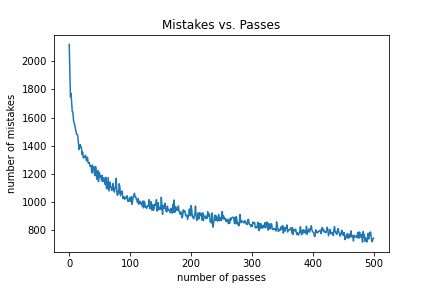
\includegraphics[width=0.7\columnwidth]{src_code/figs/ex1_result.png}
	\\
		
	Perceptron Implementation:
	\begin{lstlisting}[language=python]		
		def perceptron(
		    X: List[List[float]], 
		    y: List[int], 
		    max_pass=500
		)-> [List[float], float, List[int]]:
		    """
		    @param          X: \in R^{nxd}
		    @param          y: \in {-1,1}^n 
		    @param   max_pass: \in N
		    """
		    X = np.array(X)
		    y = np.array(y)
		    [n, d] = np.shape(X)
		    w = [0] * d # w = 0_d
		    b = 0
		    mistake = []
		    for t in range(0, max_pass): # max passes / iterations
		        mistake.append(0)
		        for i in range(0, n):
		            x_i = X[i, :]
		            if (y[i] * (np.dot(x_i, w) + b)) <= 0:
		                w = w + y[i] * x_i
		                b = b + y[i]
		                mistake[t] += 1
		    
		    return w, b, mistake
	\end{lstlisting}
\end{answer}



%%%%%%%%%%%%%%%
%%%% Ex 2 %%%%%
%%%%%%%%%%%%%%%
\newpage
\setcounter{section}{2}
\begin{exercise}[Perceptron Questions (5 pts)]{ex2}
  \begin{enumerate}
    \item   (3 pts) The perceptron algorithm makes an update every time it witnesses a mistake.
      What if it makes an update on every point, regardless of whether or not that point is correctly classified? 
      For simplicity, consider a setting where where $b$ is fixed to $0$.
      Give an example of an infinite sequence of points $(x_i, y_i)$ with the following properties:
    \begin{property-list}
      \item The sequence is strictly linearly separable with $b = 0$ (i.e., the margin is some constant $\gamma > 0$) \label{p1:b},
      \item The sequence has $\max \|x_i\|_2 \leq 1$ \label{p1:R},
      \item The modified perceptron algorithm makes \red{an infinite number of mistakes on this sequence} \label{p1:inf}. 
    \end{property-list}
    Prove that it has these properties.
      Note that the perceptron convergence theorem and the first two conditions imply that, at some point, the unmodified perceptron algorithm would only make a finite number of mistakes.

\ans{\mref{ans:2:1}} 

  \item (1 pt)  Give examples of where the perceptron algorithm converges to a 0 margin halfspace, and a \red{separate example where it converges to} a maximum margin halfspace. \red{As pointed out by some on Piazza, tech- nically, if a halfspace has 0 margin, then it would misclassify anything that still lies on the hyperplane, and the perceptron algorithm would not yet have halted. If you came up with an example that ignores these cases and halts with a point on the hyperplane, that’s fine. However, the intent was more like the following, so consider solving the problem where it converges to an arbitrarily small margin halfspace.} More precisely: for any $0 < \varepsilon < 1/2$, give a dataset (with margin at least 1) and a order in which to process the points such that the perceptron algorithm halts providing a halfspace with margin $\leq \epsilon$. \red{This problem has to do with the original perceptron, not the modified perceptron from part 1.}
    
\ans{\mref{ans:2:2}} 
  \item (1 pt) Suppose that in each iteration of the perceptron algorithm, a point is chosen uniformly at random from the dataset.
    Show how the perceptron algorithm can be viewed as an instantiation of stochastic gradient descent (SGD). 
      In particular, you must provide a loss function and a learning rate such that SGD with these parameters and perceptron are identical. 

\ans{\mref{ans:2:3}} 
  \end{enumerate}
\end{exercise}

% --- ANS --- %
\newpage
\setcounter{answer}{0}
\begin{answer}[Infinite Mistakes]{ans:2:1}
	From the \Cref{p1:inf} and \Cref{p1:b}, we may conclude the following:
	\begin{align}
			\because \quad 		& \text{mistake } \forall i, \text{ and set threshold }(\delta = 0)\\
			\therefore \quad 	& y_i (\inner{\xv_i}{\wv_{i-1}}+b) \leq 0  ,\, \forall \, i\in [1, \infty)  \\
								& \Rightarrow \wv_{i} = \wv_{i-1} + y_i \xv_i   ,\, \forall \, i\in [1, \infty) \\
			\therefore \quad 	& \wv_{k} = \wv_0 + y_1 \xv_1 + \dots + y_k \xv_k , \, \forall \, k \in [1, \infty) \\	
								& \wv_{k} = \wv_0 + \sum_{i=1}^{k} {y_i \xv_i} ,  \, \forall \, k \in [1, \infty) \\	
			\because \quad 		& \text{For simplicity, } b = 0 \\
			\therefore \quad 	& b_i = 0 ,\, \forall i\\
			\because \quad 		& \text{By convention, } \wv_0 = \bm{0} \text{ will make the first always as mistake}\\
			\therefore	\quad 	& w_k = \sum_{i=1}^{k} {y_i \xv_i}, \, \forall \, k \in [1, \infty) \\
								& y_{k+1} \inner{\xv_{k+1}}{\wv_{k}} \leq 0 \, \forall \, k \in [1, \infty) \\
			\therefore	\quad 	& \inner{ y_{k+1}\,\xv_{k+1}}{\wv_{k}} \leq 0 \\
								& \inner{ y_{k+1}\,\xv_{k+1}}{\sum_{i=1}^{k} {y_i \xv_i}} \leq 0 \\
			\because	\quad	& \text{Let } \av_i = y_i \, \xv_i ,\, \forall \, i\in [1, \infty) \\
			\therefore	\quad 	& \inner{\av_{k+1}}{\sum_{i=1}^{k} {\av_i}} \leq 0 \Rightarrow \sum_{j=1}^{d}{\left({a_{k+1,j}}\,\sum_{i=1}^{k}{{a_{i,j}}}\right)} \leq 0   \Rightarrow \sum_{j=1}^{d}\sum_{i=1}^{k}{a_{k+1,j}}\,{{a_{i,j}}} \leq 0 \label{eqn:a1:condition}
	\end{align}
	Hence:
	\begin{align}
			\therefore \quad		& \text{if } \quad \mathcal{D} = \left\{(\xv_i, y_i) : \sum_{j=1}^{d}\sum_{i=1}^{k}{a_{k+1,j}}\,{{a_{i,j}}} \leq 0, \, \av_i = y_i \, \xv_i , \,  i\in [1, \infty) \right\} \\ 
								& \rightarrow \textbf{Make mistakes on infinity many points}
	\end{align}
	From the \Cref{p1:R}, we may add an additional constraint on the example:
	\begin{equation}
		\sum^{d}_{j=1}{\xv_{ij}^2} \leq 1 \Rightarrow \sum^{d}_{j=1}{a_{ij}^2} \leq 1
	\end{equation}
	Hence, in order to satisfy all three properties, the dataset would be:
	\begin{equation}
		\mathcal{D} = \left\{(\xv_i, y_i) : \sum_{j=1}^{d}\sum_{i=1}^{k}{a_{k+1,j}}\,{{a_{i,j}}} \leq 0 , \, \sum^{d}_{j=1}{a_{i,j}^2} \leq 1 , \, \av_i = y_i \, \xv_i , \,  i\in [1, \infty) , \, y_i \in \{1, -1\} \right\}
	\end{equation}	
	
	\begin{alert}
		There are infinity many examples for this question. Here, we will mathematically derive one with assumptions.	
	\end{alert}

	For simplicity, let's consider a 2D case (\Cref{a1:2d}), which allows us to visualize geometrically, since $w_i^T \av_i = |w_i||\av_i| cos(\theta_{w_i,a_i})$. The thought process here is that if we make all labels as $+1$ (\Cref{a1:label}), then $a_i = x_i$ and $w_{i+1} = w_i + x_i$, which will simplifies many things. In order to ensure the linearly separable property, we can assume all the points are on the right half of the plane and may only include one side of the vertical axis (\Cref{a1:rhd}). 

	Let's summarize up these assumptions:
	\begin{assumption-list}
		\item \Cref{p1:R} $\Rightarrow \|x_i\|_2 \leq 1$	 \label{a1:l2}
		\item 2-D data: $d = 2$ \label{a1:2d}
		\item $y_i = 1 \, \forall i$ \label{a1:label}
		\item All the points are on the right hand plane: $a_{i,1} \geq 0$ \label{a1:rhd}
	\end{assumption-list}

	Hence, from \Cref{a1:2d}, we may simplify \Cref{eqn:a1:condition} to:
	\begin{align}
		\sum_{j=1}^{d=2}\sum_{i=1}^{k}{a_{k+1,j}}\,{{a_{i,j}}} & \leq 0 \\
		a_{k+1,1}\,\sum_{i=1}^{k}{{a_{i,1}}} + a_{k+1,2}\,\sum_{i=1}^{k}{{a_{i,2}}} & \leq 0 \\
		a_{k+1,1}\,\sum_{i=1}^{k}{{a_{i,1}}} & \leq -a_{k+1,2}\,\sum_{i=1}^{k}{{a_{i,2}}}
	\end{align}

	Expanding per $(k+1)$:
	\begin{align}
		k+1 = 1	\quad & 0  \leq 0\\
		k+1 = 2	\quad & a_{2,1}\,(a_{1,1})  \leq -a_{2,2}\,(a_{1,2})\\
		k+1 = 3	\quad & a_{3,1}\,(a_{1,1} + a_{2,1})  \leq -a_{3,2}\,(a_{1,2} + a_{2,2})\\
		k+1 = 4	\quad & a_{4,1}\,(a_{1,1} + a_{2,1} + a_{3,1})  \leq -a_{4,2}\,(a_{1,2} + a_{2,2} + a_{3,2})\\
		\vdots
	\end{align}
	
	From this inequality, we can see the solution would be alternating in quadrant 2 and 4. 
	
	In addition, 
	\begin{align}
		\because \qquad & w_i^T \av_i = |w_i||\av_i| cos(\theta_{w_i,a_i}) \quad w_i^T\av_i \leq 0\\
		\therefore \qquad & \pi \geq \theta_{w_i,a_i} \geq \frac{\pi}{2}, \forall \theta_{w_i,a_i} \in [0, \pi]
	\end{align}
	This would ensure all points locate on one side of the plane, and makes mistakes.
	
	Let's draw out the concept in 2D:

	Initially, $w_0$ starts from the origin. Updating $w_{i+1} = w_i + \av_i$ essentially means $w_i$ vector keeps accumulates the $\av_i$. If the $w_i$ vector forms an angle larger than or equal to 90 degree, it guarantee it makes a mistake. \Cref{p1:inf} indicates an infinity mistakes, but permits some mistakes in between. Hence, the goal is to make this aggressive updating method make mistakes and never converges. 
	
	Say if we assume there exists repetitive series of points, that ensures the last point return back to the starting axis, but also guarantee makes an angle larger or equal than 0 all the time between the last point and the prior weight before updating. 
	
	As a result, we shall try to make a set of three vectors that can bring the ${w_{3n}, n\in \mathbb{Z}}$ back to the x-axis ($w_{3n, 2} = 0$), and we want $w_{3n-1, 2}$ and $\av_{3n}$ form an angle larger or equal than zero ($\theta_{3n-1 \rightarrow 3n} = 0$)
	
	For simplicity, let's start with a 45 degree angle ray sourced from the origin and intersect with $R$ (L2 norm boundary), where, we obtain first point $\av_1 = \left(\frac{1}{\sqrt{2}}, \frac{1}{\sqrt{2}}\right)$.
	
	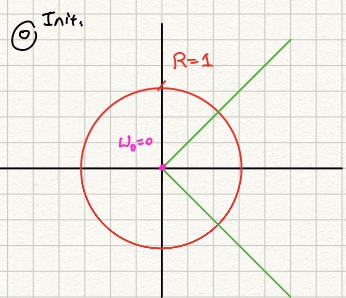
\includegraphics[width=0.45\columnwidth]{Fig/Q2-1-0.png}\quad
	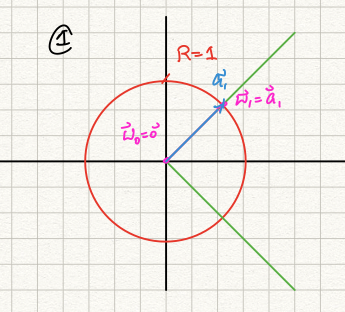
\includegraphics[width=0.4\columnwidth]{Fig/Q2-1-1.png}

	Hence, the second point has to be in the green region in quadrant 2, so that it forms an angle larger than 90 degree. In addition, we want the updated $w_2$ point fall in quadrant 4, so that it can be pulled back to x-axis with the third point in quadrant 2 ($a_{22} + a_{12} < 0$). For simplicity, we can assume a point that forms a 60 degree from the y axis with an l2 norm of 1. (You may pick any points from this region.) As a result, we compute $\av_2 = (\frac{1}{\sqrt{2}}, -\frac{1}{\sqrt{2}})$.

	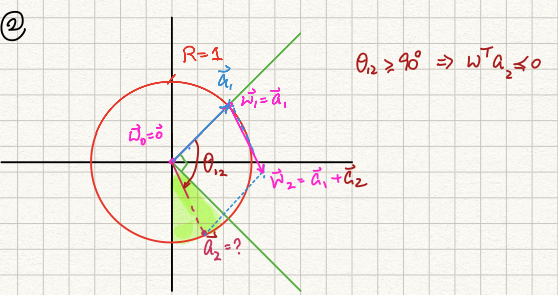
\includegraphics[width=0.8\columnwidth]{Fig/Q2-1-2.png}
	
	Now, we shall pull the weight vector back to x-axis. Hence, $a_{12} + a_{22} + a_{32} = 0$, resulting $a_{32} = \frac{\sqrt{3}}{2} - \frac{1}{\sqrt{2}}$. Most important, we need to make sure this vector $\av_{3}$ would form an angle larger than 90 degree. Since the weight vector $w_2$ will always fall below the x-axis, hence, we shall make every third point locates on positive y-axis ($a_{31} = 0$), so that it guarantees a minimum of 90 degree as $i \rightarrow \infty$. Hence, $\av_{3} = (0, \frac{\sqrt{3}}{2} - \frac{1}{\sqrt{2}})$.
	
	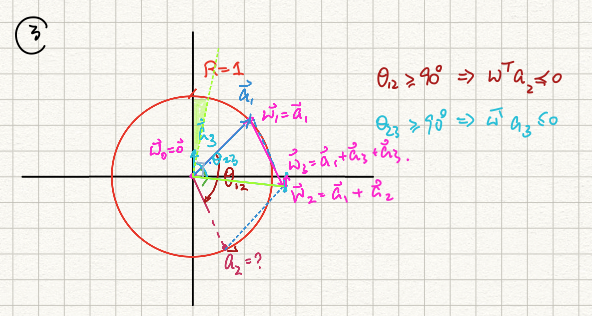
\includegraphics[width=0.8\columnwidth]{Fig/Q2-1-3.png}

	Recall $\xv_i=\av_i, y_i = 1$, therefore, we have obtained the infinity sequence:
	\begin{remark}[Final Derived Three-Point Example of an infinite sequence of points]{r1}
	\begin{equation}
		(\xv_{i}, y_{i}) =
		\begin{cases}
				((\frac{1}{\sqrt{2}}, \frac{1}{\sqrt{2}}), 1)  \quad & i= 3n + 1\\
				((\frac{1}{2}, -\frac{\sqrt{3}}{2}), 1) & i= 3n + 2 \\
				((0, \frac{\sqrt{3}}{2} - \frac{1}{\sqrt{2}}), 1) & i= 3n + 3
		\end{cases}
		,\quad n \in \mathbb{Z}
	\end{equation}		
	\end{remark}
	
	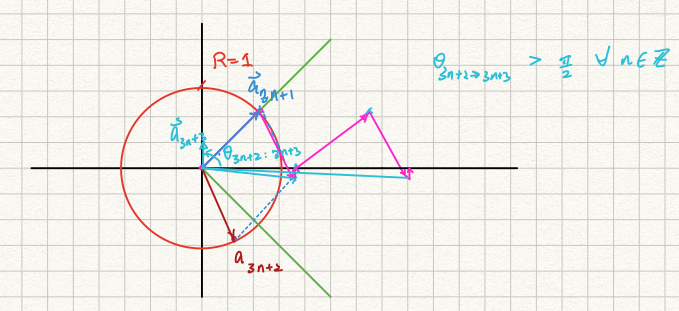
\includegraphics[width=0.8\columnwidth]{Fig/Q2-1-n.png}
	
	By observation, this repeated series will satisfies three properties from \Cref{p1:b}, \Cref{p1:R}, and \Cref{p1:inf}. Now, let's formerly prove it does indeed meet all properties:
	\begin{proof}[\Cref{p1:b} - Strictly Linearly Separable]{proof1}
		Since all labels are +1, and all data points are asymmetric, hence the data $\mathcal{D}$ is strictly linear separable with $b=0$.
		
		And the algorithm shall only make the first mistake in the ordinary perceptron with $b=0$, simply updating $w$ and $b$ to $w=(1/\sqrt{2},1/\sqrt{2}), b=0$, and then halt update. Hence, there exists $w=(1/\sqrt{2},1/\sqrt{2}), b=0$ such that $\forall i, \av^T_i w \geq s \geq 0 $. As a result, we conclude the dataset is truly strictly linearly separable.
	
		As shown in the graph below, there would exist some hyperplane, where all points on one side of the hyperplane through the origin with $\gamma > 0, b=0$.
		
		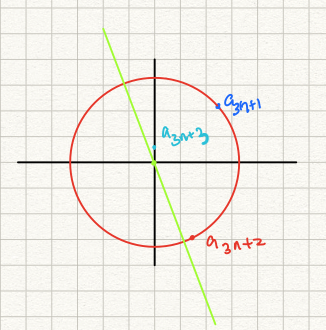
\includegraphics[width=0.4\columnwidth]{Fig/Q2-1-proof-sls.png}
		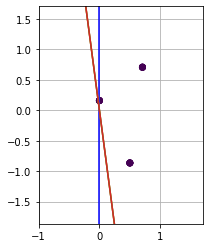
\includegraphics[width=0.35\columnwidth]{Fig/Q2-1-sls}
	\end{proof}
	\begin{proof}[\Cref{p1:R} - max $||x_i||_2 \leq 1$]{proof2}
		\begin{align}
			\because \quad & \|\av_{3n+1}\|_2 = 1 \quad \|\av_{3n+2}\|_2 = 1 \quad \|\av_{3n+3}\|_2 = \frac{\sqrt{3}}{2} - \frac{1}{\sqrt{2}} \quad  \forall n \in \mathbb{Z}\\
			\therefore \quad & \|x_i\|_2  = \|a_i\|_2 \leq 1 , \, \forall i \in \mathbb{Z}
		\end{align}
	\end{proof}
	\begin{proof}[\Cref{p1:inf}: infinite number of mistakes]{proof3}
		We can guarantee the angle formed between every third point and prior weight vector would be larger or equal than 90 degree.
		As the figure below shown, the angle $\theta{w_{3n+2}\rightarrow\av_{3n+3}} \geq \frac{\pi}{2}, \forall n \in \mathbb{Z}$.
		
		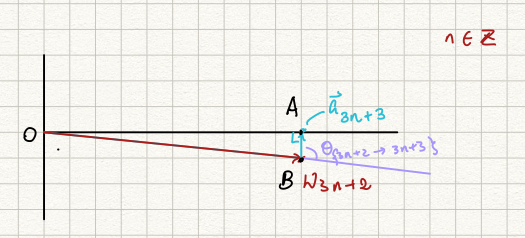
\includegraphics[width=0.8\columnwidth]{Fig/Q2-1-proof}

	\end{proof}
	
	\begin{note}[Interesting Conclusion]{green!20!pink}{note:2}
		Interestingly to note, for given any repeated set of points, as long as we ensure the last point $\av_k$ will make $w_k = w_{k-1} + \av_k$ back to x-axis and form an 90 degree or larger angle with with prior weight $w_{k-1}$. 
		
		For a 2 point series case in 2D, it is much simpler, simply any arbitrary first point in quadrant 1, and a vector on negative y-axis that will bring the first point back to x-axis:
	\begin{remark}[Generalized Two-point Solution of an infinite sequence of points]{r2gen}
	\begin{equation}
	    (\xv_i, y_i) = \begin{cases}
	    	(\xv_{2n+1},y_{2n+1}) = ((x_{2n+1, 1}, x_{2n+1, 2}), 1) \\
	    	(\xv_{2n+2},y_{2n+2}) = ((0, - x_{2n+1, 2}), 1)
	    \end{cases}
	    \quad 
	    x_{2n+1, 1} \in \mathbb{R^+}, \, x_{2n+1, 2} \in \mathbb{R} , \, n \in \mathbb{Z}
	\end{equation}
	\end{remark}
	
	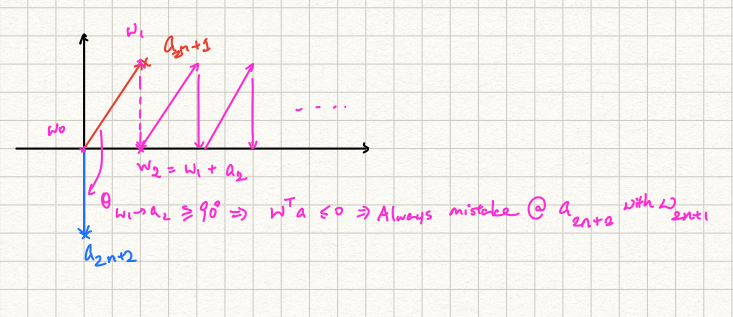
\includegraphics[width=0.8\columnwidth]{Fig/Q2-1-2point}

	For example:
	\begin{remark}[Two-point Example of an infinite sequence of points]{r2}
	\begin{equation}
		(\xv_{i}, y_{i}) =
		\begin{cases}
				((1,1), 1)  \quad & i= 2n + 1\\
				((0 , -1), 1) \quad & i= 2n + 2 \\
		\end{cases}
		,\quad n \in \mathbb{Z}
	\end{equation}
	\end{remark}
	
	It is strictly linearly separable with $b=0$:
	
	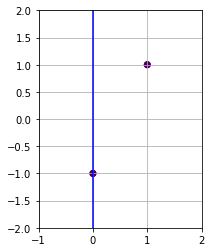
\includegraphics[width=0.3\columnwidth]{Fig/Q2-1-2pt-0}
	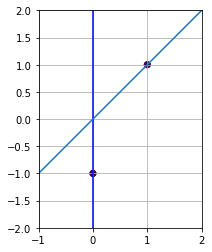
\includegraphics[width=0.3\columnwidth]{Fig/Q2-1-2pt-1}
	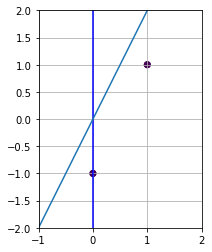
\includegraphics[width=0.3\columnwidth]{Fig/Q2-1-2pt-2}

	\end{note}

	\textbf{Q.E.D.}
\end{answer}

% --- ANS --- %
\newpage
\begin{answer}[Margin]{ans:2:2}
	\textbf{a. Example for $\varepsilon$ margin halfspace:}\\
	{
		It happens when an arbitrary working hyperplane is formed biased towards the last mistaken points. 
		
		Simplest Example: \\
		$(x_i, y_i) = \begin{cases} ((2, 2), 1) & i = 2n + 1 \\ ((-0.5, -0.5), -1) & i = 2n + 2 \end{cases}, \forall n \in \mathbb{Z}$
				
		
		Proof:
		
		Iteration 1: Since $y_1(\inner{w_0}{x_1} + b_0) = 0 \leq 0$, $\Rightarrow \quad w_1 = w_0 + y_i x_i = (2,2)$ and $b_1 = b_0 + y_1 = 1$
		
		Iteration 2: Since $y_2(\inner{w_1}{x_2} + b_1) = -1 * (\inner{(-0.5,-0.5)}{(2,2)} + 1) = 1 > 0$, $\Rightarrow \quad$ Do not update
		
		Iteration 3: Since $y_3(\inner{w_2}{x_3} + b_2) = 1 * (\inner{(2,2)}{(2,2)} + 1) = 9 > 0$, $\Rightarrow \quad$ Do not update
		
		Iteration 2i: As stated in Iteration 2

		Iteration 3i: As stated in Iteration 3
		
		Hence, it will never update after the first update.
		
		The converged hyperplane is defined by $w=(2,2), b=1$
		
		Hence, we may compute the margin: $\gamma = 0.5/\sqrt{2} = 0.3535 < 1/2 $
		
		And, the max geometric margin: $\hat{\gamma} =  \| (2,2) - (-0.5,-0.5)\| = 3.5355 > 1$
		
		Hence, in this case, the margin obtained is smaller than the max possible geometric margin.
		
		$\qquad\qquad$Initial Hyperplane $\qquad\qquad\qquad\rightarrow\qquad$  Final Hyperplane
		
		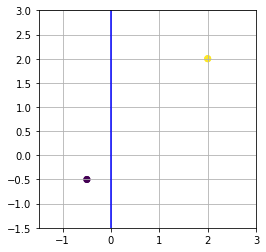
\includegraphics[width=0.4\columnwidth]{Fig/Q2-2-a1.png}
		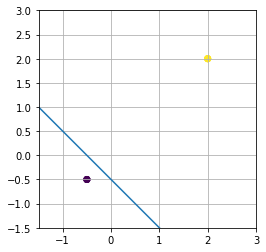
\includegraphics[width=0.4\columnwidth]{Fig/Q2-2-a2.png}
	}
	\\\\
	\clearpage
	\textbf{b. Example for a maximum margin halfspace:}\\
	{
		It happens when $\gamma = R = \underset{i}{max}||a_i||_2$,\\
		hence, all the data points are concentrated on two symmetrical points with opposing label. \\
		It would also make one mistake $\lim_{\gamma \rightarrow R}(\frac{R}{\gamma})^2 = 1$ \\
		Example: $(x_i, y_i) = (((-1)^{i}, 0), (-1)^{i})$, $\gamma = R = \underset{i}{max}||a_i||_2 = 1$\\
		
		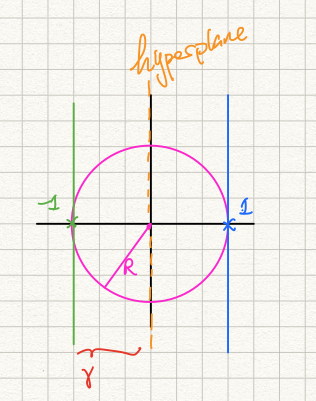
\includegraphics[width=0.4\columnwidth]{Fig/Q2-2.png}
		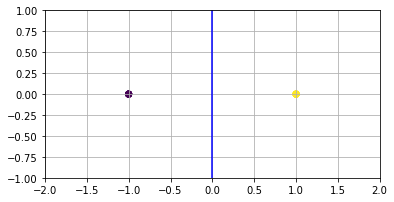
\includegraphics[width=0.4\columnwidth]{Fig/Q2-2-b.png}
	}

%	ican see how this can be a bit confusing. Let me denote two related but distinct meanings of margin.
%The margin of a *hyperplane with respect to a dataset* is the minimum distance from the hyperplane to any point in the dataset.
%The margin of a *dataset* is the maximum possible margin of a hyperplane with respect to the dataset. Stated a different way: if a dataset is strictly separable, there are many possible hyperplanes that could separate it. Choose the hyperplane which maximizes the distance to the closest point. That distance to the closest point is the margin of the dataset.
%So in some sense, the problem asks you to find the worst possible separating hyperplane, and the best possible separating hyperplane, where worst and best is measured in terms of the margin of the hyperplane with respect to the dataset.
%And you caught me on one point: technically, if the hyperplane we output has margin 0, then it would make a mistake on one of the points (based on the definition we used in class), and it wouldn't have converged. I'm going to make a clarification to the assignment saying that if this makes you uncomfortable, construct an example where the margin is some value ε, for any given ε>0.
\end{answer}

% --- ANS --- %
\newpage
%	(1 pt) Suppose that in each iteration of the perceptron algorithm, a point is chosen uniformly at random from the dataset.
%    Show how the perceptron algorithm can be viewed as an instantiation of stochastic gradient descent (SGD). 
%      In particular, you must provide a loss function and a learning rate such that SGD with these parameters and perceptron are identical. %
%\clearpage
\begin{answer}[SGD]{ans:2:3}
% Reference:
% * https://www.cs.cmu.edu/~avrim/598/chap6only.pdf
% * https://www.shivani-agarwal.net/Teaching/CIS-520/Spring-2019/Lectures/Reading/19-online-learning.pdf
% http://web.mit.edu/6.S097/www/resources/L01.pdf
% https://gluon.mxnet.io/chapter02_supervised-learning/perceptron.html
	The goal for Stochastic Gradient Descent (SGD) is to learn a model to minimize the loss $\ell(\wv;\xv_i,y_i)$ over a training set $\mathcal{D} = {(\xv_i,y_i)}$. Similarly, we can consider the minimization is related to a linear mode with form of $f_w(x)=\inner{\wv}{x}$. Hence:
	\begin{equation}
		\underset{w}{\min} \frac{1}{n} \sum_{i=1}^n{\ell(\wv;\xv_i,y_i)} = \underset{w}{\min}  \frac{1}{n} \sum_{i=1}^n{\ell(\inner{\wv}{\xv_i},y_i)} 
	\end{equation}
	
	Then SGD basically updates the weight vector $\wv_t$ by performing an approximate gradient descent:
	\begin{equation}
		\wv_{t+1} \leftarrow \wv_t - \eta_t \,\nabla_{\wv}\ell(\wv;\xv_i,y_i) \label{eqn:q23:sgd_update}
	\end{equation}

    Recall the perceptron update:
    \begin{align}
    	\text{if} \quad & y_i(\inner{\wv_i}{\xv_i} + b_i) \leq 0 \Rightarrow (y_i\inner{\wv_i}{\xv_i} + y_i\,b_i) \leq 0 \label{eqn:q23:if} \\
    	\text{then}\quad &  \wv_{i+1} \leftarrow \wv_i + y_i \xv_i \label{eqn:q23:wv} \\
    								& b_{i+1} \leftarrow b_i + y_i \label{eqn:q23:b}	
    \end{align}
    
    As \Cref{eqn:q23:if} stated, when $y(\inner{\wv}{\xv} + b)$ is larger than zero, the system does not update. It updates only when $y(\inner{\wv}{\xv} + b)$ is less than zero (when there is a mistake).
    
    Hence, it is equivalent to update when the $- y(\inner{\wv}{\xv} + b)$ is larger than zero. This can be the loss function we try to minimize for when the term is larger than zero.
    
	Hence, we may assume the loss function as:
    \begin{equation}
    	\ell(\wv;\xv_i,y_i) = \max{(0, - y_i\,\inner{\wv}{\xv_i} - y_i \, b)}
    \end{equation}

    Conveniently, this result a gradient:
    \begin{equation}
    	\nabla_{\wv,b} \ell(\wv;\xv_i,b;y_i) = \frac{\partial \max{(0, - y_i\,\inner{\wv}{\xv_i} - y_i \, b)}}{\partial \wv}
    \end{equation}
    
    We may also separate them into to two distinct components for $w$ and $b$:
    \begin{align}
    	\nabla_{\wv} & \ell(\wv;\xv_i,y_i) = \max{(0, -y_i \xv_i)}\\
    	\nabla_{b}   & \ell(b;y_i) = \max{(0, -y_i)}
    \end{align}

	Since the data at each iteration '$t$' of SGD is randomly selected from the dataset $\mathcal{D}$, hence we may replace $(y_i,\xv_i)$ with sampled dataset $(y_t,\xv_t)$, which is characterized in a Stochastic GD instead of the GD method. 
	
	As a result, the SGD update function (\Cref{eqn:q23:sgd_update}) becomes:
	\begin{align}
		\wv_{t+1} &\leftarrow \wv_t - \eta_t \,\nabla_{\wv}\ell(\wv;\xv_i,y_i) = \wv_t - \eta_t \, \max{(0, -y_i \xv_i)} = \max{(\wv_t, \wv_t + \eta_t y_i \xv_i)} \label{eqn:q23:result}\\
		b_{t+1} &\leftarrow b_t - \eta_t \,\nabla_{b}\ell(b;y_i) = b_t - \eta_t \, \max{(0, -y_i)} = \max{(b_t,  b_t + \eta_t y_i)}  \label{eqn:q23:result2}
	\end{align}

	As \Cref{eqn:q23:result} and \label{eqn:q23:result2} stated, the SGD formulation stated above returns exact result as the update function for the weight in the perceptual algorithm (\Cref{eqn:q23:wv} and \Cref{eqn:q23:b} respectively), when the learning rate is the step size $\eta_t = 1$. It either maintain the current $\wv_t$ and $b_t$, or update towards a better location to minimize the loss function (in another word, when it makes a mistake).

	In conclusion, we may conclude the perceptron algorithm can be viewed as an instantiation of stochastic gradient descent (SGD), with:
	\begin{itemize}
		\item a loss function:  $\ell(\wv;\xv_i,y_i) = \max{(0, - y_i\,\inner{\wv}{\xv_i} - y_i \, b)}$
		\item a learning rate: 	$\eta_t = 1$
	\end{itemize}
\end{answer}

%%%%%%%%%%%%%%%
%%%% Ex 3 %%%%%
%%%%%%%%%%%%%%%
\newpage
\setcounter{section}{3}
\begin{exercise}[Regression Implementation (8 pts)]{ex3}
Recall that ridge regression refers to
\begin{align}
\min_{\wv\in \RR^d, b\in \RR} ~ \overbrace{\underbrace{\tfrac{1}{2n} \|X \wv+ b\one - \yv\|_2^2}_{\mbox{error}} + \lambda \|\wv\|_2^2}^{\mbox{loss}},\label{ex31:loss}
\end{align}
where $X \in \RR^{n \times d}$ and $\yv \in \RR^n$ are the given dataset and $\lambda > 0$ is the regularization hyperparameter.

\begin{enumerate}
\item (1 pt) Show that the derivatives are
\begin{align}
\frac{\partial}{\partial\wv} &=  \tfrac1n X^\top (X\wv + b\one - \yv) + 2 \lambda \wv\\
\label{eq:b}
\frac{\partial}{\partial b} &= \tfrac1n \one^\top (X\wv + b\one - \yv).
\end{align}

    \ans{\mref{ans:3:1}} 

\item (2 pts) Implement the gradient descent algorithm for solving ridge regression. The following \red{incomplete} pseudo-code may of help.

Test your implementation on the Boston \href{http://lib.stat.cmu.edu/datasets/boston}{\textsf{\magenta{housing}}} dataset (to predict the median house price, \ie, $y$). Use the train and test splits provided on \href{http://www.gautamkamath.com/courses/CS480-wi2021.html}{\magenta{course website}}. Try $\lambda \in \{0, 10\}$ and report your training error, training loss and test error. [Your training loss should monotonically decrease during iteration; if not try to tune your step size $\eta$, \eg make it smaller.]

\begin{algorithm}[H]
\DontPrintSemicolon
	\KwIn{$X\in\RR^{n\times d}$, $\yv\in \RR^n$, $\wv_0=\zero_d$, $b_0=0$, $\mathsf{max\_pass} \in \mathds{N}$, $\eta > 0$, $\mathsf{tol} > 0$}

	\KwOut{$\wv, b$}

	\For{$t=1, 2, \ldots, \mathsf{max\_pass}$ }{
		$\wv_t \gets  $

		$b_t \gets $

		\If(\tcp*[f]{can use other stopping criteria}){$\|\wv_{t} - \wv_{t-1}\|  \leq \mathsf{tol}$}{
			\textbf{break}
		}
	}

	$\wv \gets \wv_t, ~ b \gets b_t$
	\caption{Gradient descent for ridge regression.}
	\label{alg:rr}
\end{algorithm}

    \ans{\mref{ans:3:2}}

For the next part, you may use the Python package scikit-learn.

\item (5 pts) Train (unregularized) linear regression, ridge regression, and lasso on the mystery datasets A, B, and C on the course website (using X\_train and Y\_train for each dataset).
  For ridge regression and lasso, use parameters $1$ and $10$ (note that you will have to divide these by $n$ for lasso in scikit-learn -- why?).
  Report the average mean squared error on the test set for each method.
  Which approach performs best in each case?
    Plot the five parameter vectors obtained for each dataset on the same histogram, so they're all visible at once (change the opacity setting for the bars if necessary): specifically, for each parameter vector, plot a histogram of its value in each coordinate.
    Given which approach performs best, and how its parameter histogram looks, how do you suspect the true parameter vector and responses might have been generated?

  \ans{\mref{ans:3:3}}
\end{enumerate}
\end{exercise}

% --- ANS --- %
\newpage
\setcounter{answer}{0}
\begin{answer}[Derivatives Derivation]{ans:3:1}
	Let's simplify the loss function (in \Cref{ex31:loss}) with some sub-group functions:
	\begin{align}
		f_{error}(X, \wv, \yv, b) &= X \wv+ b\one - \yv \\
		f_{reg}(\wv) &= \wv 
	\end{align}
	We will also apply partial derivative to these sub-group functions with respect to $\wv$ and $b$:
	\begin{align}
		\frac{\partial f_{error}(X, \wv, \yv, b)}{\partial \wv} 
			&= \frac{\partial (X \wv+ b\one - \yv)}{\partial \wv} \\
			&= \frac{\partial (X \wv)}{\partial \wv} 
			= 
			\begin{bmatrix}
				\frac{\partial (\xv_1^T \wv)}{\partial \wv} \\
				\frac{\partial (\xv_2^T \wv)}{\partial \wv} \\
				\vdots \\
				\frac{\partial (\xv_n^T \wv)}{\partial \wv} \\
			\end{bmatrix} 
			= 
			\begin{bmatrix}
				\xv_1 & \xv_2 & \dots & \xv_n
			\end{bmatrix}
			= X^T
		\\
		\frac{\partial f_{error}(X, \wv, \yv, b)}{\partial b} 
			&= \frac{\partial (X \wv+ b\one - \yv)}{\partial b} \\
			&= \frac{\partial (b \one)}{\partial 1} 
			= \one^T
		\\
		\frac{\partial f_{reg}(\wv)}{\partial \wv} &= 1 
		\\
		\frac{\partial f_{reg}(\wv)}{\partial b} &= 0
	\end{align}
	Hence, the loss function now becomes:
	\begin{equation}
		\ell(X, \wv, \yv, b) = \frac{1}{2n} \| f_{error}(X, \wv, \yv, b)\|_2^2 + \lambda \| f_{reg}(\wv) \|_2^2
	\end{equation}
	Now, we may apply 1st order derivatives with Chain Rule:
	\begin{align}
		\frac{\partial \ell(X, \wv, \yv, b)}{\partial \wv} 
			&= \frac{\partial \frac{1}{2n} \| f_{error}(X, \wv, \yv, b)\|_2^2 + \lambda \| f_{reg}(\wv) \|_2^2
}{\partial \wv} \\
			&=  \frac{1}{2n} \cdot 2 \frac{\partial f_{error}}{\partial \wv} \cdot f_{error} +  \lambda \cdot 2 \cdot \frac{\partial f_{reg}}{\partial \wv} \cdot f_{reg} \\
			&= \frac{1}{n} \cdot X^T \cdot (X \wv+ b\one - \yv) + 2 \lambda \cdot 1 \cdot \wv \\
			&= \tfrac1n X^\top (X\wv + b\one - \yv) + 2 \lambda \wv
	\end{align}
	\begin{align}
		\frac{\partial \ell(X, \wv, \yv, b)}{\partial b} 
			&= \frac{\partial \frac{1}{2n} \| f_{error}(X, \wv, \yv, b)\|_2^2 + \lambda \| f_{reg}(\wv) \|_2^2
}{\partial b} \\
			&=  \frac{1}{2n} \cdot 2 \cdot \frac{\partial f_{error}}{\partial b} \cdot f_{error} +  0\\
			&= \frac{1}{n} \cdot \one^T \cdot (X \wv+ b\one - \yv) \\
			&= \tfrac1n \one^\top (X\wv + b\one - \yv)
	\end{align}
\textbf{Q.E.D.}
\end{answer}

% --- ANS 3.2 --- %
\newpage
\begin{answer}[]{ans:3:2}
For the test, we have setup tuning parameters as following:
\begin{lstlisting}[language=python]
	COMMON_MAX_PASS     = 10000
	COMMON_ETA          = 1e-7 # >0
	COMMON_TOLERANCE    = 5e-5 # >0
	COMMON_ERR_TOL      = 35.8 # Disable: None
\end{lstlisting}
\vspace{-20pt}
With the default termination criterion (which terminates when the slope of $w$ below certain threshold), the algorithm seems to perform similarly as Trial 1 and 2 in the table below.

Hence, we modified the stopping criterion so that it terminates when training error reaches below the given tolerance. As Trial 3 and 4 in the table below shown, the trial with $\lambda = 10$ takes longer passes with better performance on test dataset with lower test error. We do observer both trial 2 and 4 has better performance than without regularization term ($\lambda = 0$).

\begin{center}
	\begin{tabular}{p{0.5cm} p{1cm} p{1cm} p{6cm} p{1.5cm} p{1.5cm} p{1.5cm}} \hline
		%% Header
		Trial & $\lambda$ & Passes & Training Progress & Training Error & Training Loss & Test Error  
		\\ \hline
		%% Content
		1 & 0 & 136 & \raisebox{-105px}{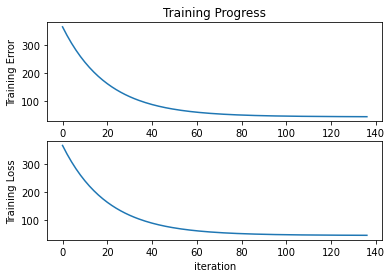
\includegraphics[height=112px]{src_code/figs/ex3-2_training_progress_lam=0.png}} & 44.42208 & 44.42208 & 108.42167
		\\ \hline
		2 & 10 & 136 & \raisebox{-105px}{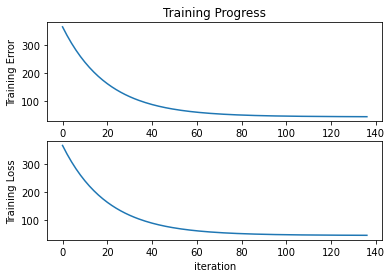
\includegraphics[height=112px]{src_code/figs/ex3-2_training_progress_lam=10.png}} & 44.42367  & 44.44802 & 108.39676
		\\ \hline
		3 & 0 & 2899 & \raisebox{-105px}{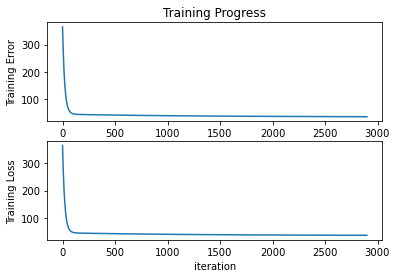
\includegraphics[height=112px]{src_code/figs/ex3-2_training_progress_lam=0,ES.png}} & 35.79958 & 35.79958 & 49.89885
		\\ \hline
		4 & 10 & 2911 & \raisebox{-105px}{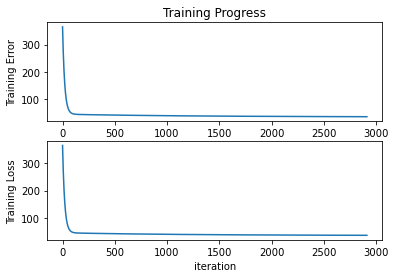
\includegraphics[height=112px]{src_code/figs/ex3-2_training_progress_lam=10,ES.png}} & 35.79973 & 35.84981 & 49.88967
      \\ \hline
	\end{tabular}
\end{center}


The complete algorithm is completed as shown below:

\begin{algorithm}[H]
\DontPrintSemicolon
	\KwIn{$X\in\RR^{n\times d}$, $\yv\in \RR^n$, $\wv_0=\zero_d$, $b_0=0$, $\mathsf{max\_pass} \in \mathds{N}$, $\eta > 0$, $\mathsf{tol} > 0$}

	\KwOut{$\wv, b$}

	\For{$t=1, 2, \ldots, \mathsf{max\_pass}$ }{
		
		$\wv_t \gets \tfrac1n X^\top (X\wv + b\one - \yv) + 2 \lambda \wv $

		$b_t \gets \tfrac1n \one^\top (X\wv + b\one - \yv)$

		\If(\tcp*[f]{can use other stopping criteria}){$\|\wv_{t} - \wv_{t-1}\|  \leq \mathsf{tol}$}{
			\textbf{break}
		}
	}

	$\wv \gets \wv_t, ~ b \gets b_t$
	\caption{Completed Pseudocode Gradient descent for ridge regression.}
	\label{alg:rr}
\end{algorithm}

The equivalent code implementation is as shown below:


	\begin{lstlisting}[language=python]		
		def gradient_descent_ridge_regression_training(
		    X: List[List[float]], 
		    y: List[float], 
		    # Configuration with Default Settings
		    max_pass: int   = 500,
		    eta: float      = 0.3, # >0
		    tol: float      = 0.1, # >0
		    lamb: float     = 0,   # Try \in {0,10}
		    error_tol: Optional[float] = None,
		)-> [List[float], float, Dict]:
		    """
		    @param          X: \in R^{nxd}
		    @param          y: \in R^n 
		    @param   max_pass: \in N
		    @param        eta: step size
		    @param        tol: tolerance
		    @param       lamb: regulation weight '\lambda'
		    """
		    XT = X
		    X = np.transpose(XT)
		    y = np.array(y)
		    [n, d] = np.shape(X) 
		    w = np.zeros(d) # w = 0_d
		    b = 0
		    mistake = []
		    # optimization: pre-compile
		    div = 1/n 
		    # logger
		    training_log = {
		        "t" : [],
		        "w" : [],
		        "b" : [],
		        "training_error": [],
		        "training_loss": [],
		    }
		    # training
		    for t in range(0, max_pass): # max passes / iterations
		        pw = copy.deepcopy(w)
		        # update:
		        f_err = ( np.dot(X, w) + b - y ) # pred - y
		        dw = div * np.dot(XT, f_err) + 2 * lamb * w
		        db = div * np.sum(f_err) # 1^T f_err
		        w = w - eta * dw
		        b = b - eta * db
		        # compute loss and error:
		        error = div / 2 * (np.linalg.norm(f_err) ** 2)
		        loss = error + lamb * (np.linalg.norm(w) ** 2)
		        # log progress:
		        training_log["t"].append(t)
		        training_log["w"].append(w)
		        training_log["b"].append(b)
		        training_log["training_error"].append(error)
		        training_log["training_loss"].append(loss)
		        # stopping criteria:
		        if error_tol is None:
		            if np.linalg.norm(pw - w) <= tol: # can use other stopping criteria
		                break # STOPPING
		        else:
		            if error <= error_tol:
		                break # STOPPING
		    
		    return w, b, training_log
	\end{lstlisting}
    
\end{answer}

% --- ANS 3.3 --- %
\newpage
\begin{answer}[]{ans:3:3}
%  For ridge regression and lasso, use parameters $1$ and $10$ (note that you will have to divide these by $n$ for lasso in scikit-learn -- why?)
	To throughly compare the lasso and ridge regression methods, we will have to divide these alpha parameters ($1$ and $10$) by $n$ for lasso in scikit-learn. This is mainly caused by the difference in objective function in scikit-learn. Specifically, the objective for the lasso incorporates the sample size $n$ as the denominator of the mean squared error \cite{web:scikit:lasso}, whereas, the objective for the ridge regression does not take into account this term \cite{web:scikit:ridge-regression}. Hence, the regulation term $\alpha$ shall also divide by the sample size $n$ in the lasso to match up with the ridge regression, so that both algorithm has similar regulation effects.

%	 Train (unregularized) linear regression, ridge regression, and lasso on the mystery datasets A, B, and C on the course website (using X\_train and Y\_train for each dataset).
%  Report the average mean squared error on the test set for each method.
%    Plot the five parameter vectors obtained for each dataset on the same histogram, so they're all visible at once (change the opacity setting for the bars if necessary): specifically, for each parameter vector, plot a histogram of its value in each coordinate.
	Test results are tabulated here:
	\begin{center}
	\begin{tabular}{p{1.5cm} p{4.5cm} p{4.5cm} p{4.5cm}} \hline
		%% Header
		Methods & Dataset A & Dataset B & Dataset C
		\\ \hline
		%% Content
		Linear & MSE = 3.24740 & MSE = 2.74268 & MSE = 506.37271
		\\ \hline
		Ridge 1 & MSE = 3.13939 & MSE = 2.61621 & MSE = 505.27731
		\\ \hline
		Ridge 10 & MSE = 2.77803 & MSE = 2.05971 & MSE = 515.89174
		\\ \hline
		Lasso 1 & MSE = 3.02040 & MSE = 2.26517 & MSE = 1.87747
		\\ \hline
		Lasso 10 & MSE = 3.60263 & MSE = 1.80967 & MSE = 1.35256
		\\ \hline
		(Hist.) & \raisebox{-100px}{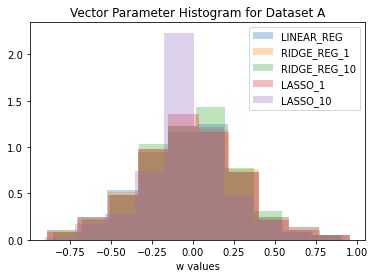
\includegraphics[height=100px]{src_code/figs/ex3-3_hist_A}} & \raisebox{-100px}{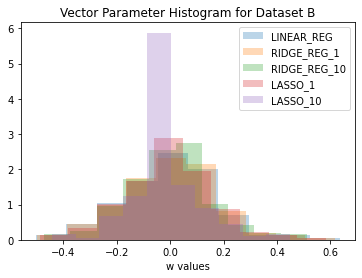
\includegraphics[height=100px]{src_code/figs/ex3-3_hist_B}} & \raisebox{-100px}{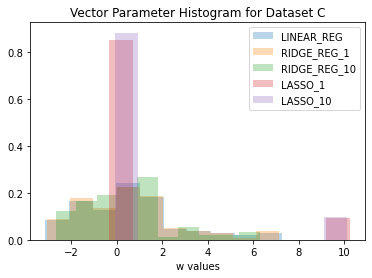
\includegraphics[height=100px]{src_code/figs/ex3-3_hist_C}}
		\\ \hline
		(Hist.) & \raisebox{-100px}{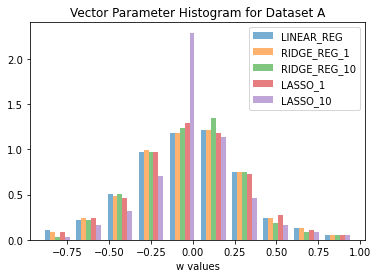
\includegraphics[height=100px]{src_code/figs/ex3-3_hist_A_sep}} & \raisebox{-100px}{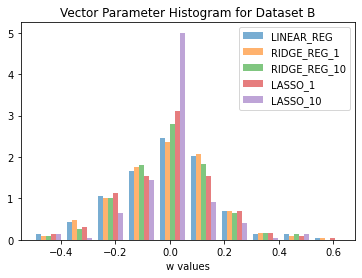
\includegraphics[height=100px]{src_code/figs/ex3-3_hist_B_sep}} & \raisebox{-100px}{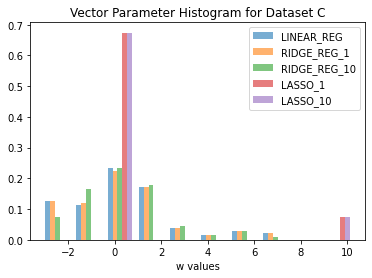
\includegraphics[height=100px]{src_code/figs/ex3-3_hist_C_sep}}
		\\ \hline
	\end{tabular}
	\end{center}
	
%  Which approach performs best in each case?
	It appears that "Ridge 10" performs the best in dataset A, and "Lasso 10" performed the best for both dataset B and C.
%    Given which approach performs best, and how its parameter histogram looks, how do you suspect the true parameter vector and responses might have been generated?
The classic ridge regression uses L2 regularization, whereas the Lasso uses the L1 regularization. Hence, the L2 norm will place the outsize penalty on large components of the weight vector, hence, the histogram of L2 (Ridge Regression) would be more evenly distributed across many features. L1 norm leads to a concentrate weights on a small set of features by clearing other weights to zero, which leads to a concentrated and spiky histogram with respect to ridge regression model. The L1 behaviour is also known as feature extraction.

As we can see from the datasets, as the alpha increases, the Lasso becomes more concentrated. In dataset C, the "Lasso 10" and "Lasso 1" has some large weights at $10$, where classical regression and ridge regression failed to register. For this particular dataset C, Lasso performed the best, hence, we may conclude the dataset C is quite sparse and complex. In the case of sparse data, rigid and classical would be normalized. Hence, we may see the rigid regression with high L2 regularization make worser prediction on the dataset. Whereas, the L1 regularization in Lasso helps to compensate the sparsity and complexity. It is also possible that the ridge regression and linear modelling over-fit the training dataset, while the lasso will reduce this over-fit by feature extraction. 

For dataset A, the Ridge with large coefficient performed the best, whereas the lasso with the large coefficient performed the worst. This indicates the dataset A has a significant multi-collinearity. The ridge is capable to shrink the model complexity and multi-collinearity. Whereas, the lasso would reduce the complexity by feature extraction but suffers if the data has a significant multi-collinearity. The lasso would select one of the dominant feature to enhance and attenuates all other features. Hence, the lasso with high regulation factor in this case performed the worst, due to feature losses (or over-simplified).

For dataset B, it is observed that the ridge perform better as the coefficient increases, and the lasso with a large gain perform the best overall. This indicates the dataset has a small degree of complexity.


As per requested on Piazza to think about how we generate the response $Y$ from the true weight distribution $\hat{W}$, and based on the above observation and analysis, we may suspect the response is generated from three different $\hat{W}$ with different distribution model:

The dataset A might generate the weight based on a Gaussian distribution centered at zero mean, resulting a smooth curved histogram centered at $w=0$. In addition, there are additive noises centered at zero mean with small variance introduced when computing the response. As a result, the ridge performs the best, since there exists multiple features that are correlated at the same time. 

The dataset B might be based on a double exponential distribution centered at zero, since the tip of the predicted weight appeared to be quite spiky, and there exists a significant feature resulting a better performance in Lasso.

The dataset C might be based on a double exponential distribution centered at zero as well, but with an additive noise centered at 10, resulting a sparse response $Y$.
\end{answer}


%%%%%%%%%%%%%%%
%%%% Ex 4 %%%%%
%%%%%%%%%%%%%%%
\newpage
\setcounter{section}{4}
\begin{exercise}[An Alternative to Least Squares? (3 pts)]{ex4}
Suppose we are in a setting with a dataset $X \in \mathbb{R}^{n \times d}$, and labels are generated according to $Y = XW + \varepsilon$, where $W \in \mathbb{R}^d$, $Y \in \mathbb{R}^n$, and $\varepsilon \in \mathbb{R}^n$ is a random vector, where all entries are independent random variables with $0$ mean and variance $\sigma^2$ (you can imagine Gaussian, but it isn't necessary).
    As we saw in class, the least-squares solution $\hat W$ can be written as $\hat W = (X^T X)^{-1}X^T Y$ -- this is a linear transformation of the response vector $Y$.
    Consider some \emph{different} linear transformation $\left((X^T X)^{-1}X^T + N\right)Y$, where $N \in \mathbb{R}^{d \times n}$ is a non-zero matrix.
\begin{enumerate}
  \item (1 pt) Show that the expected value of this linear transformation is $(I_d + NX)W$.
    Conclude that its expected value is $W$ if and only if $NX = 0$. (1 pt)

    \ans{\mref{ans:4:1}} 
  \item (2 pts) Compute the covariance matrix of this linear transformation when $NX = 0$, and show that it is equal to $\sigma^2 (X^T X)^{-1} + \sigma^2 NN^T$.
    Since the former term is the covariance of the least squares solution\footnote{Verify this for yourself, but no need to submit it.} and the latter matrix is positive semi-definite, this implies that this alternative estimator only increased the variance of our estimate.

    \ans{\mref{ans:4:2}} 
\end{enumerate}
\end{exercise}
% --- ANS 4.1 --- %
\setcounter{answer}{0}
\begin{answer}[]{ans:4:1}
	Let us name this linear transformation as $\hat{W}$.
	\begin{align}
		E[\hat{W}] 
			&= E\left[ \left((X^T X)^{-1}X^T + N\right)Y \right]\\
			&= E\left[ \left((X^T X)^{-1}X^T + N\right) \left(XW + \varepsilon \right) \right]\\
			&= E\left[ \left((X^T X)^{-1}X^T + N\right)XW + \left((X^T X)^{-1}X^T + N\right)\varepsilon \right]\\
			&= E\left[ \left((X^T X)^{-1}X^T + N\right)XW \right] + E\left[ \left((X^T X)^{-1}X^T + N\right)\varepsilon \right]\\
			&= E\left[ \left(\cancelto{I_d}{(X^T X)^{-1}X^TX} + NX\right)W \right] + E\left[ \left((X^T X)^{-1}X^T + N\right)\right] \cancelto{0}{E\left[\varepsilon \right]}\\
			&= E\left[ (I_d + NX)W \right] \\
			&= (I_d + NX)W 
	\end{align}
	We may also prove the expected value is $W$ if and only if $NX = 0$:
	\begin{align}
		E[\hat{W}] 
			&= (I_d + NX)W \\
			&= W + NXW \\
		E[\hat{W}] - W &= NXW \\
		\text{If } & NXW \neq 0 \Rightarrow E[\hat{W}] - W \neq 0 \Rightarrow E[\hat{W}] \neq W \\
		\text{If } & NXW = 0 \Rightarrow E[\hat{W}] - W = 0 \Rightarrow E[\hat{W}] = W \\
		\therefore & E[\hat{W}] = W \, \textbf{ iff } NXW = 0
	\end{align}
	\textbf{Q.E.D.}
\end{answer}
% --- ANS 4.2 --- %
\newpage
\begin{answer}[]{ans:4:2}
% https://theclevermachine.wordpress.com/2013/01/14/derivation-the-covariance-matrix-of-an-ols-estimator-and-applications-to-gls/	for OLS
	Similar to \Cref{ans:4:1}, we may derive $\hat{W}$ and $(\hat{W} - W)$:
	\begin{align}
		\because \qquad \hat{W} &= \left((X^T X)^{-1}X^T + N\right)XW + \left((X^T X)^{-1}X^T + N\right)\varepsilon \\
			&= \cancelto{I_d}{(X^T X)^{-1}X^TX}W + \cancelto{0}{NX}W + (X^T X)^{-1}X^T \varepsilon + N \varepsilon \\
			&= W + (X^T X)^{-1}X^T \varepsilon + N \varepsilon \\
		\therefore \, \hat{W} - W &= (X^T X)^{-1}X^T \varepsilon + N \varepsilon
	\end{align}
	
	We may now compute the covariance matrix:
	\begin{align}
		\Sigma &= E\left[ (\hat{W} - W) (\hat{W} - W)^T \right] \\
			&= E\left[ \left((X^T X)^{-1}X^T \varepsilon + N \varepsilon \right) \left((X^T X)^{-1}X^T \varepsilon + N \varepsilon\right)^T \right] \\
			&= E\left[\left((X^T X)^{-1}X^T \varepsilon + N \varepsilon \right) \left(\varepsilon^TX(X^T X)^{-1} + \varepsilon^T N^T \right)\right]\\
			&= E\left[(X^T X)^{-1}X^T \varepsilon \, \varepsilon^TX(X^T X)^{-1} + N \varepsilon \, \varepsilon^TX(X^T X)^{-1} + \varepsilon^T  N^T  \, (X^T X)^{-1}X^T + N \varepsilon \, \varepsilon^T  N^T \right]\\
			&=  E\left[(X^T X)^{-1}(X^TX) \varepsilon \varepsilon^T (X^T X)^{-1} + NX\varepsilon \, \varepsilon^T(X^T X)^{-1} + N^T X^T \varepsilon^T  \, (X^T X)^{-1} + N \varepsilon \, \varepsilon^T  N^T \right]\\
			&=  E\left[\cancelto{I_d}{(X^T X)^{-1}(X^TX)} \varepsilon \varepsilon^T (X^T X)^{-1} + \cancelto{0}{NX}\varepsilon \, \varepsilon^T(X^T X)^{-1} + \cancelto{0}{(NX)^T} \varepsilon^T  \, (X^T X)^{-1} + N \varepsilon \, \varepsilon^T  N^T \right] \\
			&=  E\left[\varepsilon \varepsilon^T (X^T X)^{-1} + N \varepsilon \, \varepsilon^T  N^T \right]\\
			&=  E\left[\varepsilon \varepsilon^T (X^T X)^{-1}\right] +  E\left[N \varepsilon \, \varepsilon^T  N^T \right]\\
			&=  E\left[\varepsilon \varepsilon^T\right] (X^T X)^{-1} +  E\left[ \varepsilon \, \varepsilon^T\right] N  N^T \\
			&= \sigma^2(X^T X)^{-1} + \sigma^2 N  N^T 
	\end{align}
	\textbf{Q.E.D.}
	
	\begin{remark}[$\epsilon$ Term]{remark:4.5}
		$E[\varepsilon \varepsilon^T] = \sigma^2 I_d$: The covariance of additive noise term is the variance, which is $\sigma^2$ as provided \\
		$E[\varepsilon] = 0 $: The expectation of the additive noise term is the mean, which is 0 as provided
	\end{remark}

\end{answer}

%%%%%%%%%%%%%%%
%%%% Ex 5 %%%%%
%%%%%%%%%%%%%%%
\newpage
\setcounter{section}{5}
\begin{exercise}[Sample Statistics (2 pts)]{ex5}
  \begin{enumerate}
  \item (1 pt) Suppose there is a dataset $x_1, \dots, x_n$ sampled from a distribution with mean $\mu$ and variance $\sigma^2$.
    Compute the expected value of the sample mean: $\bar x = \frac{1}{n} \sum_{i=1}^n x_i$. 
    Describe any modifications that might be required to make the expected value $\mu$ (recall that $\mu$ and $\sigma^2$ are unknown). 

    \ans{\mref{ans:5:1}}
  \item (1 pt) Suppose there is a dataset $x_1, \dots, x_n$ sampled from a distribution with mean $\mu$ and variance $\sigma^2$.
    Compute the expected value of the sample variance: $\frac{1}{n} \sum_{i=1}^n \left(x_i - \bar x \right)^2$, where $\bar x$ is the sample mean from the previous part.
    Describe any modifications that might be required to make the expected value $\sigma^2$ (recall that $\mu$ and $\sigma^2$ are unknown). 
    
    \ans{\mref{ans:5:2}} 
\end{enumerate}
\end{exercise}
% --- ANS 5.1 --- %
\setcounter{answer}{0}
\begin{answer}[]{ans:5:1}
	%	https://online.stat.psu.edu/stat414/lesson/24/24.4
	\begin{align}
		E[\bar{x}] 
			&= E\left[ \frac1n \sum_{i=1}^n x_i \right] \\
			&= \frac1n \sum_{i=1}^n E\left[ x_i \right] \\
		\because \quad & E[x_i] = \mu \forall i \\
			&= \frac1n \sum_{i=1}^n \mu \\
			&= \frac1n \cdot n \mu \\
			&= \mu
	\end{align}
	Hence:
	\begin{equation}
		\mu = E[\bar{x}] = E\left[ \frac1n \sum_{i=1}^n x_i \right]
	\end{equation}
	Hence, the expected value of the sample mean is $\mu$. No additional modification is required.

	\textbf{Q.E.D.}
\end{answer}
% --- ANS 5.2 --- %
\newpage
\begin{answer}[]{ans:5:2}
	% https://www.youtube.com/watch/D1hgiAla3KI	
	\begin{align}
		E\left[ \frac1n \sum_{i=1}^n (x_i - \bar{x})^2 \right] 
		&= E\left[ \frac1n \sum_{i=1}^n (x_i^2 - 2 x_i \bar{x} + \bar{x}^2) \right] \\
		&= E\left[ \frac1n (\sum_{i=1}^n x_i^2 - 2 \sum_{i=1}^n x_i \bar{x} + \sum_{i=1}^n \bar{x}^2) \right] \\
	\because \quad & \sum_{i=1}^n x_i = n \bar{x} \leftarrow \text{ as stated in \Cref{ans:5:1}}\\
	\therefore &= E\left[ \frac1n (\sum_{i=1}^n x_i^2 - 2 n \bar{x} \bar{x} + n \bar{x}^2) \right] \\	
		&= E\left[ \frac1n (\sum_{i=1}^n x_i^2 - n \bar{x}^2) \right] \\	
		&= \frac1n (\sum_{i=1}^n E\left[ x_i^2 \right] -  n E\left[\bar{x}^2 \right]) \\
	\because \quad & \text{Assume it is independent} \\
	\therefore \quad & E[x_i^2] = \sigma^2 + \mu^2 \quad E[\bar{x}^2] = \frac{\sigma^2}{n} + \mu^2\\
	\therefore	&= \frac1n \left(\sum_{i=1}^n (\sigma^2 + \mu^2) -  n (\frac{\sigma^2}{n} + \mu^2) \right) \\
		&= \frac1n \left(n (\sigma^2 + \mu^2) -  n (\frac{\sigma^2}{n} + \mu^2) \right) \\
		&= \frac1n \left(n (\sigma^2 + \mu^2 - \frac{\sigma^2}{n} - \mu^2) \right) \\
		&= \frac{n-1}{n} \sigma^2 \\
	\end{align}
	Hence, we need modification:
	\begin{equation}
		\sigma^2 = \frac{n}{n-1}  E\left[ \frac1n \sum_{i=1}^n (x_i - \bar{x})^2 \right] 
	\end{equation}
	
	The expected variance $\sigma^2$ shall be multiplying $\frac{n}{n-1}$ with the sample variance.

	In the special case of $n \rightarrow \infty$ (or simply large enough), we may assume $\sigma^2 = \lim_{n\rightarrow\infty} \frac{n}{n-1}  E\left[ \frac1n \sum_{i=1}^n (x_i - \bar{x})^2 \right] = E\left[ \frac1n \sum_{i=1}^n (x_i - \bar{x})^2 \right]$.
	
	\textbf{Q.E.D.}
\end{answer}

%%%%%%%%%%%%%%%%%%%%%%%%%%%%%%%%%%%%%%%%%%%%%%%%%%%%%%%%%%%%%%%%%%%%%%%%%%%%%%%%
%% ************************************************************************** %%
%% *                      TODO [Remove For Final Copy!]                     * %%
%% ************************************************************************** %%
%%%%%%%%%%%%%%%%%%%%%%%%%%%%%%%%%%%%%%%%%%%%%%%%%%%%%%%%%%%%%%%%%%%%%%%%%%%%%%%%
%\printlistoftodos

%%%%%%%%%%%%%%%%%%%%%%%%%%%%%%%%%%%%%%%%%%%%%%%%%%%%%%%%%%%%%%%%%%%%%%%%%%%%%%%%
%% ************************************************************************** %%
%% *                                Glossary                                * %%
%% ************************************************************************** %%
%%%%%%%%%%%%%%%%%%%%%%%%%%%%%%%%%%%%%%%%%%%%%%%%%%%%%%%%%%%%%%%%%%%%%%%%%%%%%%%%
% \clearpage
\printglossaries

%%%%%%%%%%%%%%%%%%%%%%%%%%%%%%%%%%%%%%%%%%%%%%%%%%%%%%%%%%%%%%%%%%%%%%%%%%%%%%%%
%% ************************************************************************** %%
%% *                               References                               * %%
%% ************************************************************************** %%
%%%%%%%%%%%%%%%%%%%%%%%%%%%%%%%%%%%%%%%%%%%%%%%%%%%%%%%%%%%%%%%%%%%%%%%%%%%%%%%%

% \printbibliography[heading=none]

%%%%%%%%%%%%%%%%%%%%%%%%%%%%%%%%%%%%%%%%%%%%%%%%%%%%%%%%%%%%%%%%%%%%%%%%%%%%%%%%
%% ************************************************************************** %%
%% *                               Appendices                               * %%
%% ************************************************************************** %%
%%%%%%%%%%%%%%%%%%%%%%%%%%%%%%%%%%%%%%%%%%%%%%%%%%%%%%%%%%%%%%%%%%%%%%%%%%%%%%%%
% appendices use section and subsection numbering
\clearpage
\appendix
\begin{appendices}
% INPUT UR APPENDIX
\end{appendices}

\end{document}


